\section{Referencia de la Clase Albaran\-Proveedor\-View}
\label{classAlbaranProveedorView}\index{AlbaranProveedorView@{AlbaranProveedorView}}
Muestra la ficha del albar\'{a}n de proveedor.  


{\tt \#include $<$albaranproveedorview.h$>$}

Diagrama de herencias de Albaran\-Proveedor\-View\begin{figure}[H]
\begin{center}
\leavevmode
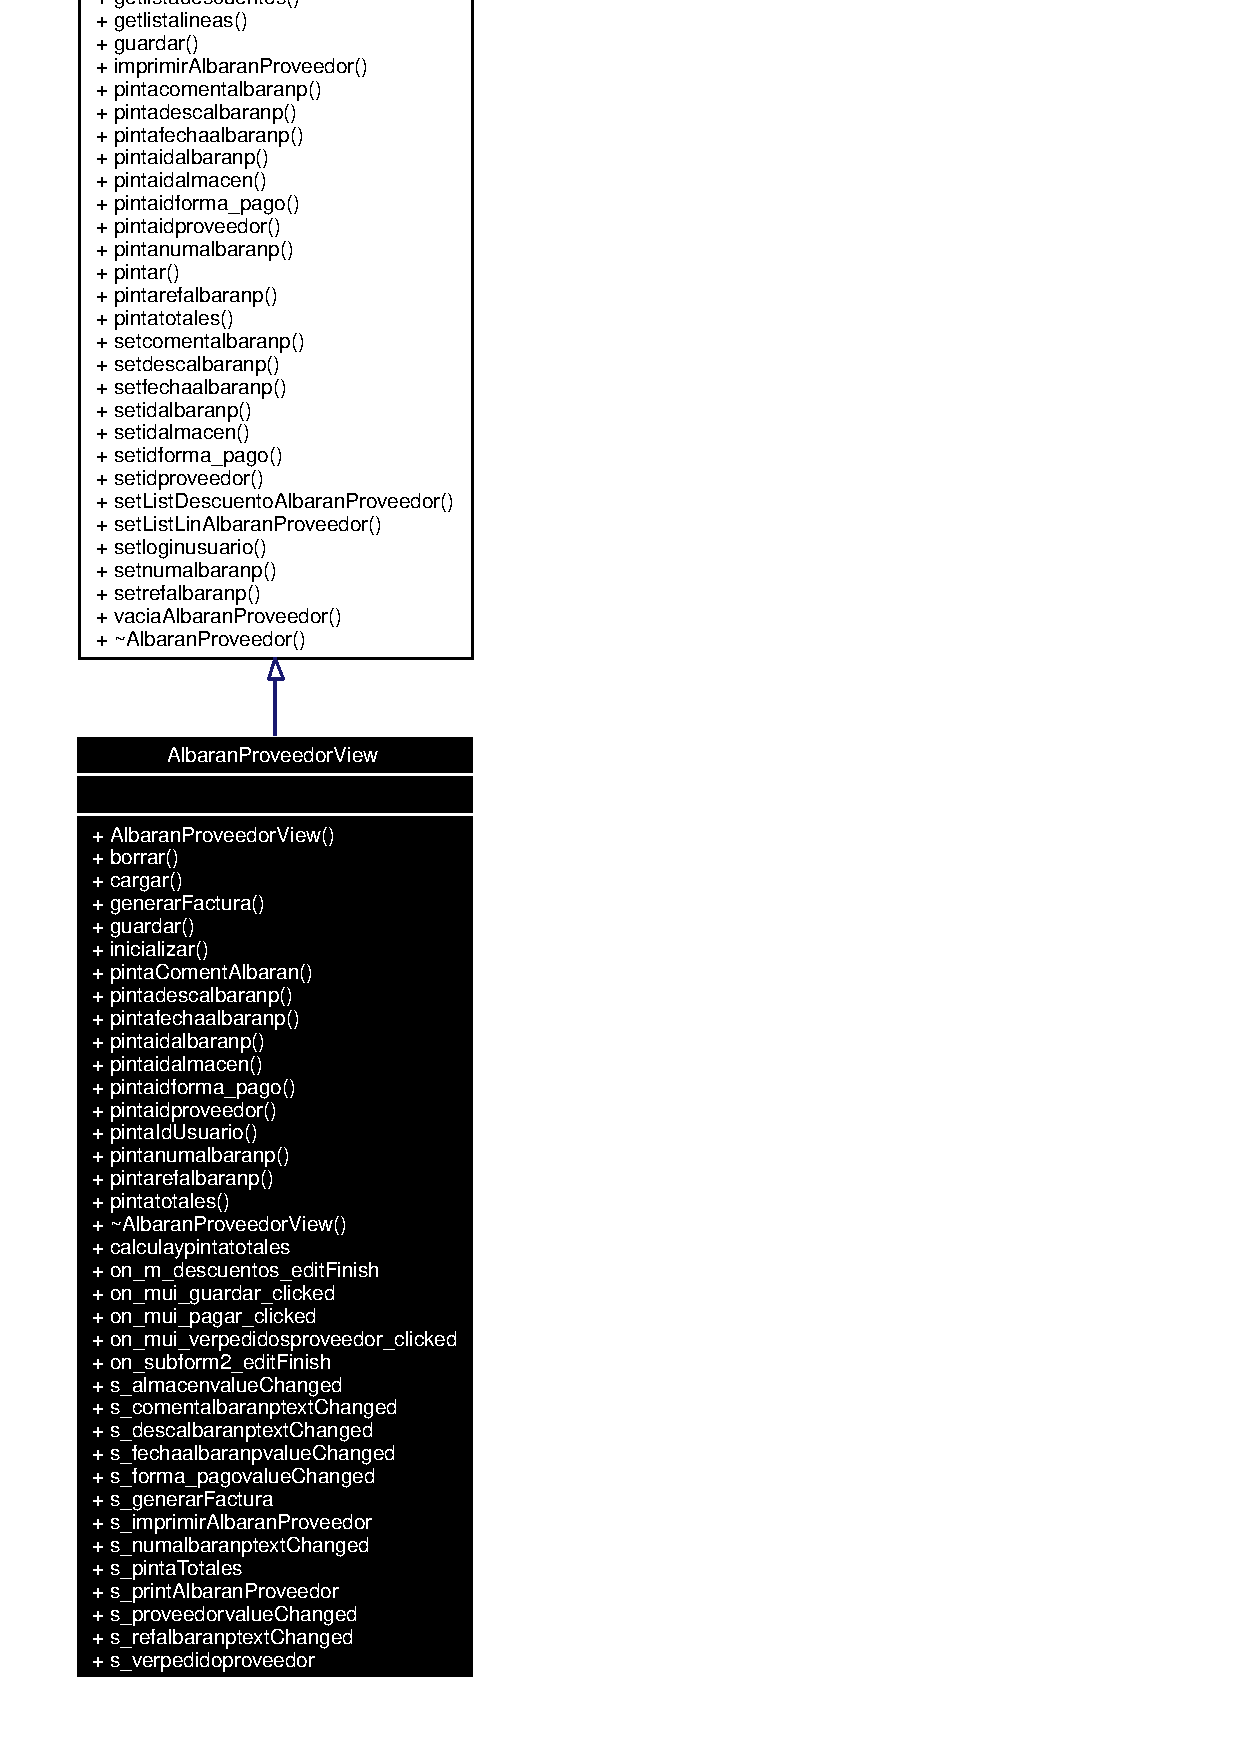
\includegraphics[width=114pt]{classAlbaranProveedorView__inherit__graph}
\end{center}
\end{figure}
Diagrama de colaboraci\'{o}n para Albaran\-Proveedor\-View:\begin{figure}[H]
\begin{center}
\leavevmode
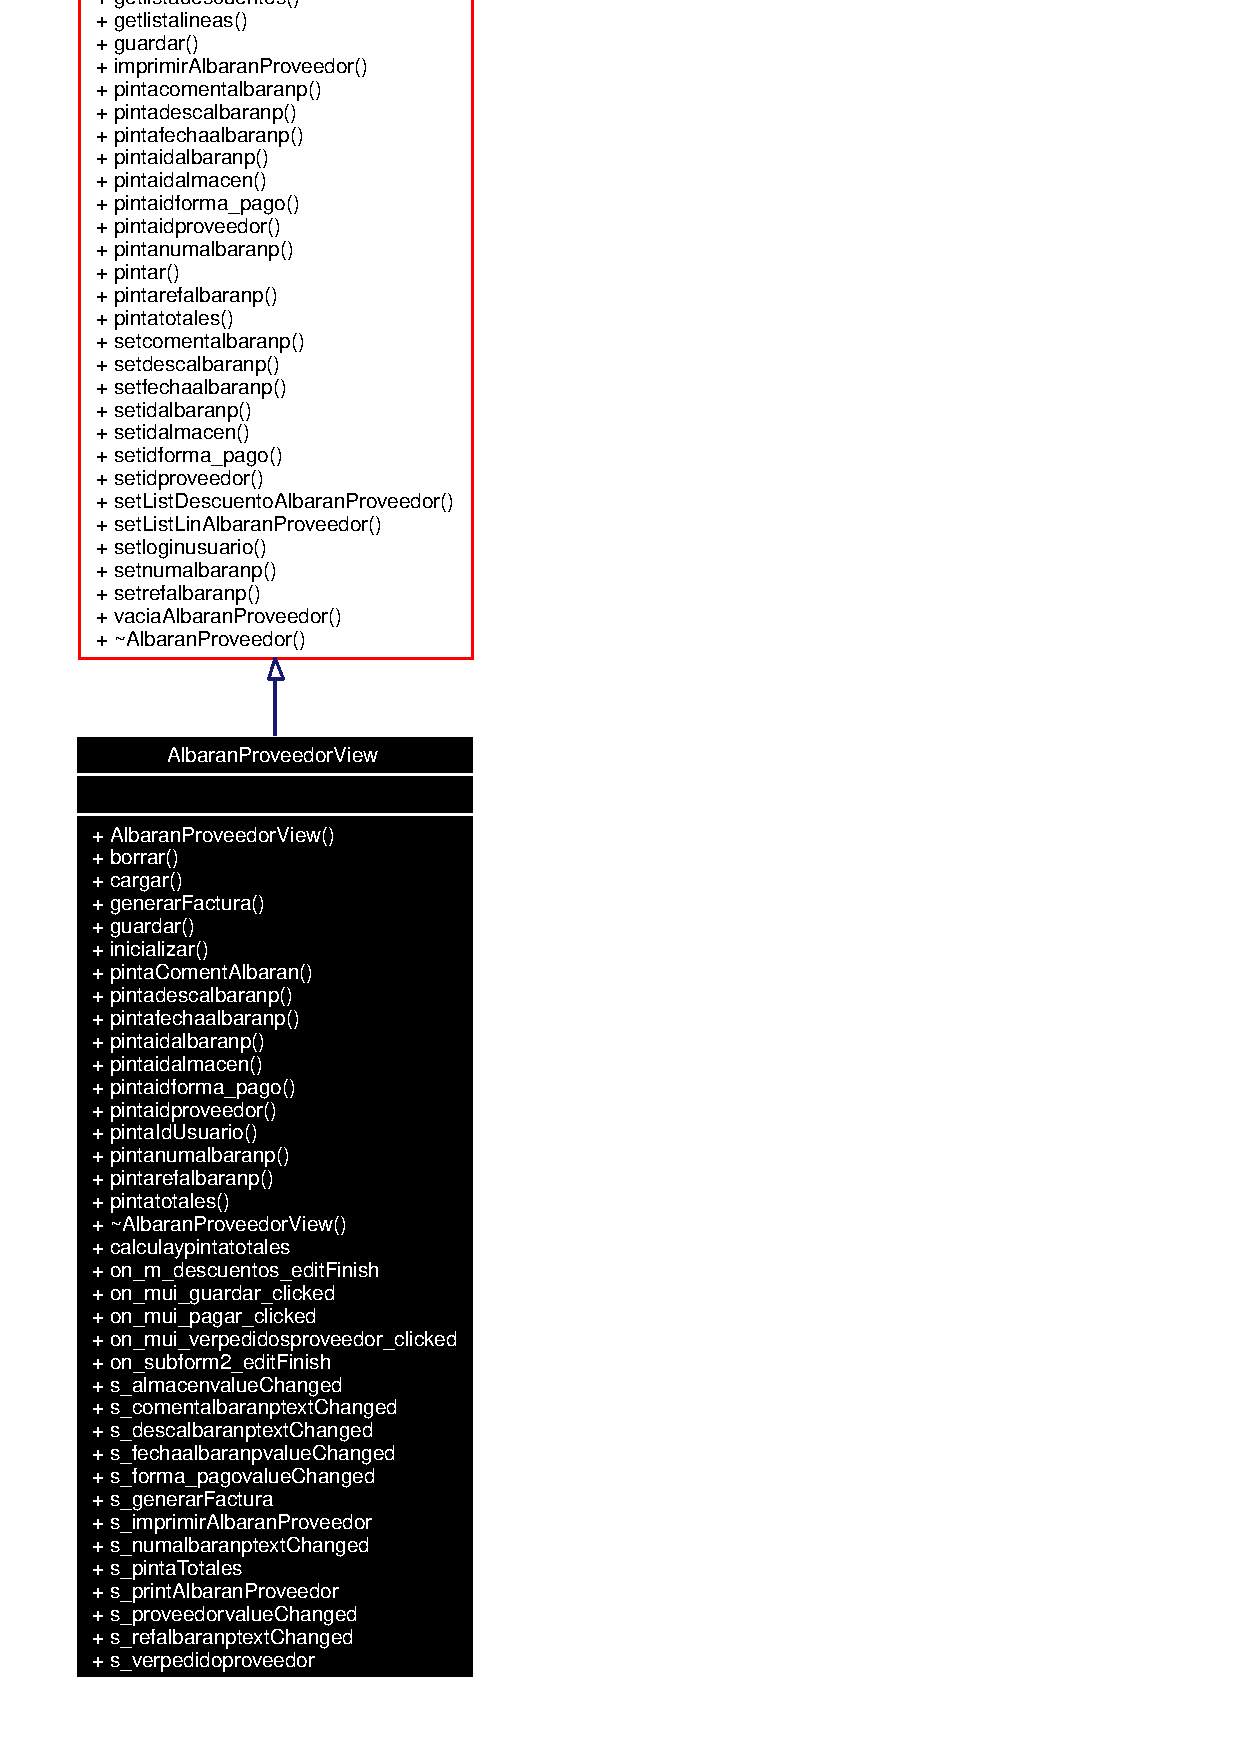
\includegraphics[width=114pt]{classAlbaranProveedorView__coll__graph}
\end{center}
\end{figure}
\subsection*{Slots p\'{u}blicos}
\begin{CompactItemize}
\item 
virtual void {\bf calculaypintatotales} ()\label{classAlbaranProveedorView_i0}

\item 
virtual void {\bf on\_\-m\_\-descuentos\_\-edit\-Finish} (int, int)\label{classAlbaranProveedorView_i1}

\item 
virtual void {\bf on\_\-mui\_\-guardar\_\-clicked} ()\label{classAlbaranProveedorView_i2}

\item 
virtual void {\bf on\_\-mui\_\-pagar\_\-clicked} ()\label{classAlbaranProveedorView_i3}

\item 
virtual void {\bf on\_\-mui\_\-verpedidosproveedor\_\-clicked} ()\label{classAlbaranProveedorView_i4}

\item 
virtual void {\bf on\_\-subform2\_\-edit\-Finish} (int, int)\label{classAlbaranProveedorView_i5}

\item 
virtual void {\bf s\_\-almacenvalue\-Changed} (QString val)\label{classAlbaranProveedorView_i6}

\item 
virtual void {\bf s\_\-comentalbaranptext\-Changed} ()\label{classAlbaranProveedorView_i7}

\item 
virtual void {\bf s\_\-descalbaranptext\-Changed} (const QString \&val)\label{classAlbaranProveedorView_i8}

\item 
virtual void {\bf s\_\-fechaalbaranpvalue\-Changed} (QString val)\label{classAlbaranProveedorView_i9}

\item 
virtual void {\bf s\_\-forma\_\-pagovalue\-Changed} (QString val)\label{classAlbaranProveedorView_i10}

\item 
virtual void {\bf s\_\-generar\-Factura} ()\label{classAlbaranProveedorView_i11}

\item 
virtual void {\bf s\_\-imprimir\-Albaran\-Proveedor} ()\label{classAlbaranProveedorView_i12}

\item 
virtual void {\bf s\_\-numalbaranptext\-Changed} (const QString \&val)\label{classAlbaranProveedorView_i13}

\item 
virtual void {\bf s\_\-pinta\-Totales} ()\label{classAlbaranProveedorView_i14}

\begin{CompactList}\small\item\em Este slot se activa cuando hay cambios en los subformularios. \item\end{CompactList}\item 
virtual void {\bf s\_\-print\-Albaran\-Proveedor} ()\label{classAlbaranProveedorView_i15}

\item 
virtual void {\bf s\_\-proveedorvalue\-Changed} (QString val)\label{classAlbaranProveedorView_i16}

\item 
virtual void {\bf s\_\-refalbaranptext\-Changed} (const QString \&val)\label{classAlbaranProveedorView_i17}

\item 
virtual void {\bf s\_\-verpedidoproveedor} ()\label{classAlbaranProveedorView_i18}

\end{CompactItemize}
\subsection*{M\'{e}todos p\'{u}blicos}
\begin{CompactItemize}
\item 
{\bf Albaran\-Proveedor\-View} ({\bf company} $\ast$, QWidget $\ast$)\label{classAlbaranProveedorView_a0}

\item 
virtual int {\bf borrar} ()\label{classAlbaranProveedorView_a1}

\item 
virtual int {\bf cargar} (QString id)\label{classAlbaranProveedorView_a2}

\begin{CompactList}\small\item\em Esta funcion carga un {\bf Albaran\-Proveedor}{\rm (p.\,\pageref{classAlbaranProveedor})}. \item\end{CompactList}\item 
void {\bf generar\-Factura} ()
\begin{CompactList}\small\item\em Se encarga de generar una facturap a partir del albaranp. \item\end{CompactList}\item 
virtual int {\bf guardar} ()\label{classAlbaranProveedorView_a4}

\begin{CompactList}\small\item\em Estos metodos deben existir para poder trabajar con la clase Ficha. \item\end{CompactList}\item 
void {\bf inicializar} ()\label{classAlbaranProveedorView_a5}

\item 
void {\bf pinta\-Coment\-Albaran} (QString val)\label{classAlbaranProveedorView_a6}

\item 
void {\bf pintadescalbaranp} (QString val)\label{classAlbaranProveedorView_a7}

\item 
void {\bf pintafechaalbaranp} (QString val)\label{classAlbaranProveedorView_a8}

\item 
void {\bf pintaidalbaranp} (QString)\label{classAlbaranProveedorView_a9}

\item 
void {\bf pintaidalmacen} (QString id)\label{classAlbaranProveedorView_a10}

\item 
void {\bf pintaidforma\_\-pago} (QString val)\label{classAlbaranProveedorView_a11}

\item 
void {\bf pintaidproveedor} (QString val)\label{classAlbaranProveedorView_a12}

\item 
void {\bf pinta\-Id\-Usuario} (QString)\label{classAlbaranProveedorView_a13}

\item 
void {\bf pintanumalbaranp} (QString val)\label{classAlbaranProveedorView_a14}

\item 
void {\bf pintarefalbaranp} (QString val)\label{classAlbaranProveedorView_a15}

\item 
void {\bf pintatotales} (Fixed, Fixed)\label{classAlbaranProveedorView_a16}

\end{CompactItemize}


\subsection{Descripci\'{o}n detallada}
Muestra la ficha del albar\'{a}n de proveedor. 



\subsection{Documentaci\'{o}n de las funciones miembro}
\index{AlbaranProveedorView@{Albaran\-Proveedor\-View}!generarFactura@{generarFactura}}
\index{generarFactura@{generarFactura}!AlbaranProveedorView@{Albaran\-Proveedor\-View}}
\subsubsection{\setlength{\rightskip}{0pt plus 5cm}void Albaran\-Proveedor\-View::generar\-Factura ()}\label{classAlbaranProveedorView_a3}


Se encarga de generar una facturap a partir del albaranp. 

Comprobamos que existe el elemento, y en caso afirmativo lo mostramos y salimos de la funcion.

Informamos de que no existe el pedido y a ver si lo queremos realizar. Si no salimos de la funcion.

Creamos la factura. 

La documentaci\'{o}n para esta clase fu\'{e} generada a partir de los siguientes archivos:\begin{CompactItemize}
\item 
albaranproveedorview.h\item 
albaranproveedorview.cpp\end{CompactItemize}
